\section{\RU{Некоторые паттерны в бинарных файлах}\EN{Some binary file patterns}}

% TODO translate

All examples here were prepared on the Windows with active code page 437 in console. % FIXME URL
Binary files internally may look visually different if another code page is set.

\subsection{Arrays}

\EN{Sometimes, we can clearly spot an array of 16/32/64-bit values visually, in hex editor.}
\RU{Иногда мы можем легко заметить массив 16/32/64-битных значений визуально, в шестнадцатеричном 
редакторе.}

% TODO translate
Вот пример массива 16-битных значений.
Мы видим что каждый первый байт в паре всегда равен 7 или 8, а второй выглядит случайным:

\begin{figure}[H]
\centering
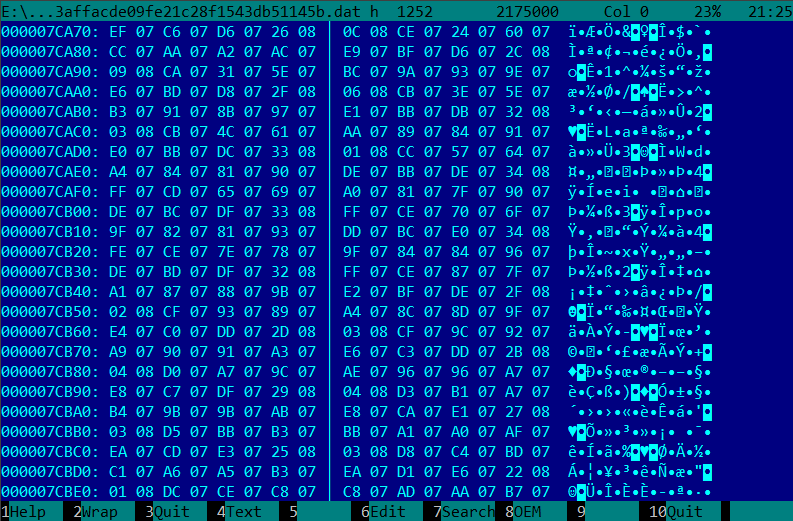
\includegraphics[scale=\NormalScale]{digging_into_code/binary/16bit_array.png}
\caption{Hiew: \EN{массив 16-битных значений}\RU{array of 16-bit values}}
\end{figure}

% TODO translate
Для примера я использовал файл содержащий 12-канальный сигнал оцифрованный при помощи 16-битного АЦП.

\index{MIPS}
\par
\EN{And here is an example of very typical MIPS code.}
\RU{А вот пример очень типичного MIPS-кода.}
\EN{As we may remember, every MIPS (and also ARM in ARM mode or ARM64) instruction has size of 32 bits (or 4 bytes), 
so such code is array of 32-bit values.}
\RU{Как мы наверное помним, каждая инструкция в MIPS (а также в ARM в режиме ARM, или ARM64) имеет 
длину 32 бита (или 4 байта),
так что такой код это массив 32-битных значений.}
\EN{By looking at this screenshot, we may see some kind of pattern.}
\RU{Глядя на этот скриншот, можно увидеть некий узор.}
\EN{Vertical red lines are added for clarity}\RU{Вертикальные красные линии добавлены для ясности}:

\begin{figure}[H]
\centering
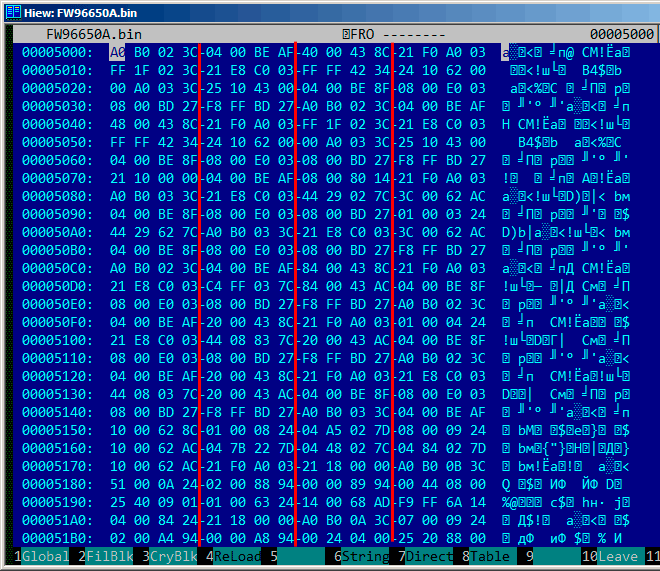
\includegraphics[scale=\NormalScale]{digging_into_code/binary/typical_MIPS_code.png}
\caption{Hiew: \EN{very typical MIPS code}\RU{очень типичный код для MIPS}}
\end{figure}

\ifx\LITE\undefined
\RU{Еще пример таких файлов в этой книге}\EN{Another example of such pattern here is book}: 
\myref{Oracle_SYM_files_example}.
\fi

\subsection{Sparse files}

This is sparse file with data scattered at relatively long distances.
Each space here is in fact zero byte (which is looks like space).
This is a file to program FPGA (Altera Stratix GX device).
Of course, files like these can be compressed easily, but formats like this one are very popular in scientific and engineering software where efficient access is important while compactness is not.

\begin{figure}[H]
\centering
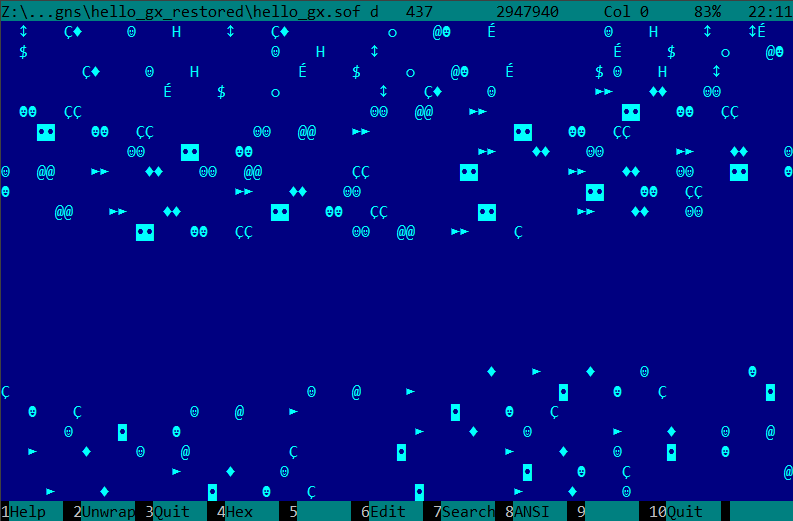
\includegraphics[scale=\NormalScale]{digging_into_code/binary/sparse_FPGA.png}
\caption{Hiew: \EN{Sparse file}\RU{...}}
\end{figure}

\subsection{Compressed file}

This file is just some compressed archive.
It has relatively high entropy (\ref{...}) and visually looks just chaotic.
This is how compressed and/or encrypted files looks like.

\begin{figure}[H]
\centering
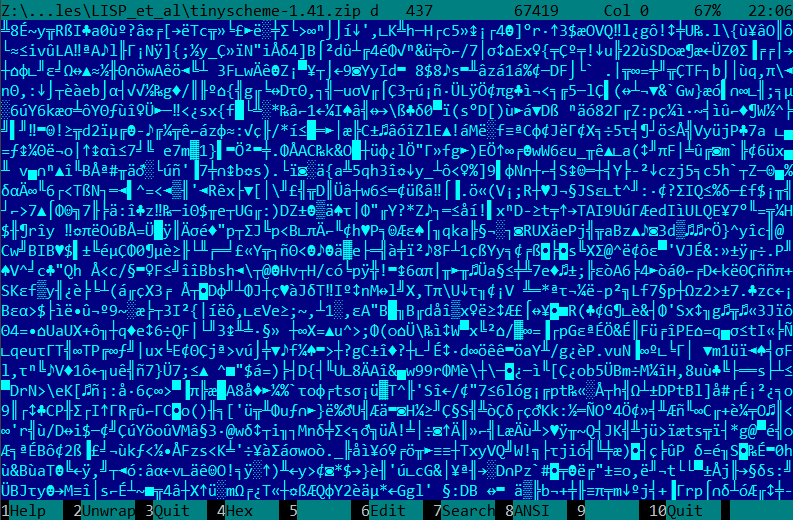
\includegraphics[scale=\NormalScale]{digging_into_code/binary/compressed.png}
\caption{Hiew: \EN{Compressed file}\RU{...}}
\end{figure}

\subsection{\ac{CDFS}}

\ac{OS} installations are usually distributed as ISO files which are copies of CD/DVD discs.
Filesystem used is named \ac{CDFS}, here is you see file names mixed with some additional data.
This can be file sizes, pointers to another directories, file attributes, etc.
This is how typical filesystems may look internally.

\begin{figure}[H]
\centering
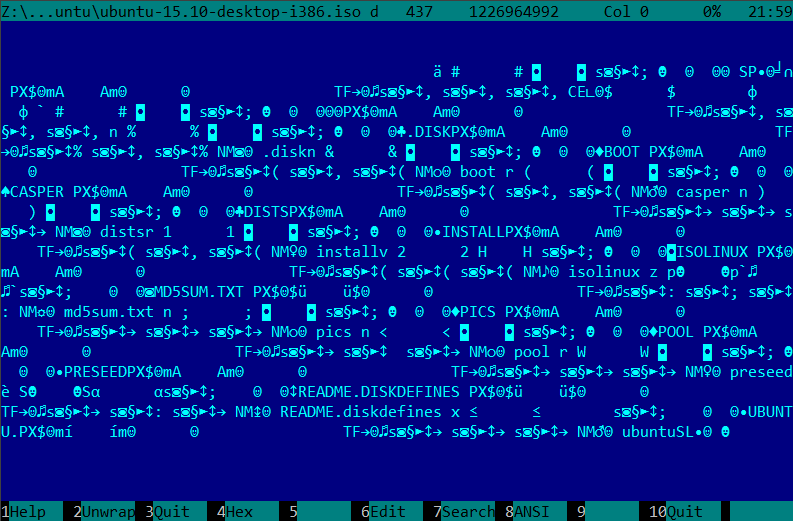
\includegraphics[scale=\NormalScale]{digging_into_code/binary/cdfs.png}
\caption{Hiew: \EN{ISO file: Ubuntu 15 installation CD\RU{...}}
\end{figure}

\subsection{32-bit x86 executable code}

This is how 32-bit x86 executable code looks like.
It has not very high entropy, so some bytes occurred more often than others.

\begin{figure}[H]
\centering
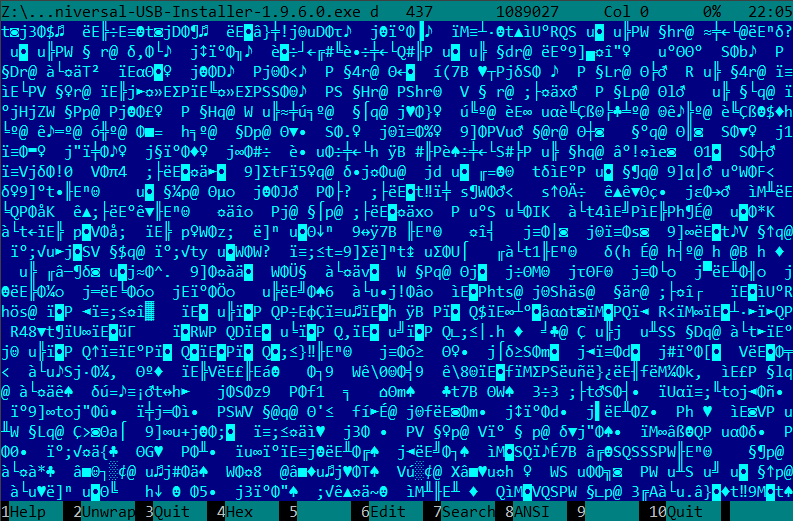
\includegraphics[scale=\NormalScale]{digging_into_code/binary/x86_32.png}
\caption{Hiew: \EN{Executable 32-bit x86 code\RU{...}}
\end{figure}

Read more about x86 statistics: \ref{}. % FIXME blog post about decryption...

\subsection{BMP files}

BMP files are not compressed, so each byte (or group of bytes) describes each pixel.
I've found this picture somewhere inside my Windows 8.1 installation:

\begin{figure}[H]
\centering

\includegraphics[scale=\NormalScale]{digging_into_code/binary/bmp.png}
\caption{\EN{Example picture}\RU{...}}
\end{figure}

You see that this picture has some pixels which probably cannot be compressed very good (around center), but there are long one-color lines at top and bottom.
Indeed, lines like these also looks as lines inside:

\begin{figure}[H]
\centering
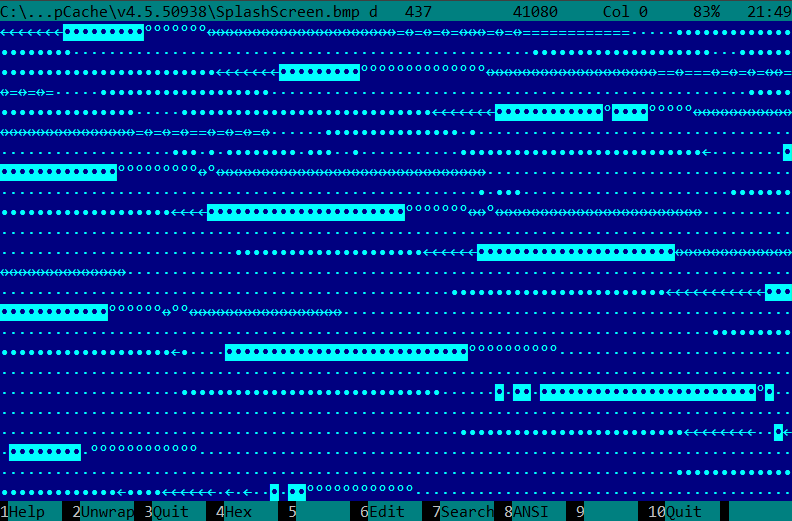
\includegraphics[scale=\NormalScale]{digging_into_code/binary/bmp_hiew.png}
\caption{Hiew: \EN{... inside}\RU{...}}
\end{figure}

